\chapter{Tổng quan và Phát biểu bài toán}
\label{ch:intro}

\section{Bối cảnh thực tiễn và Tính cấp thiết của đề tài}
Việt Nam là quốc gia có hình thể địa lý đặc thù kéo dài hơn 1.650~km theo trục Bắc -- Nam, với đường bờ biển uốn lượn dài trên 3.260~km cùng địa hình đa dạng từ vùng núi cao hiểm trở phía Bắc, các dãy đèo dốc ven dải Trường Sơn miền Trung đến vùng đồng bằng châu thổ sông Hồng và sông Cửu Long. Đặc điểm địa lý này tạo nên sự phân hóa khí hậu hết sức phức tạp: miền Bắc mang khí hậu cận nhiệt đới ẩm với mùa đông lạnh và sương muối; miền Trung thường xuyên hứng chịu bão nhiệt đới dữ dội và lũ quét; trong khi miền Nam đặc trưng bởi hai mùa mưa - nắng rõ rệt của khí hậu nhiệt đới xavan.

Các hiện tượng thời tiết cực đoan như mưa giông cục bộ cường độ lớn, gió lốc giật mạnh, sương mù dày đặc trên các cung đường đèo và ngập úng đô thị diễn ra với tần suất ngày càng dày đặc. Các điều kiện thời tiết bất lợi này làm suy giảm nghiêm trọng hệ số ma sát giữa lốp xe và mặt đường, triệt tiêu tầm nhìn quan sát của người lái xe và làm tăng đột biến nguy cơ xảy ra tai nạn giao thông \cite{andrey2003weather}. Tại Việt Nam, rủi ro này đặc biệt nghiêm trọng do đặc thù văn hóa giao thông: hơn 72 triệu xe máy đã đăng ký chiếm tới hơn 85\% tổng lưu lượng phương tiện cá nhân tham gia giao thông hàng ngày. Khác với người ngồi trong cabin ô tô khép kín, người đi xe máy hoàn toàn tiếp xúc trực tiếp với các tác động khắc nghiệt của thời tiết. Những cơn mưa rào bất chợt làm trơn trượt mặt đường, những đợt gió giật ngang trên các cây cầu vượt biển hay sương mù che khuất tầm nhìn trên các cung đèo hiểm trở như Pha Đin, Ô Quy Hồ, Hải Vân đe dọa trực tiếp đến tính mạng của hàng triệu người dân mỗi ngày.

Mặc dù điều kiện khí tượng có ảnh hưởng sống còn đến an toàn di chuyển, người tham gia giao thông tại Việt Nam hiện nay vẫn chưa có một công cụ số tích hợp nào có khả năng tính toán lộ trình trực tiếp dựa trên trường dữ liệu thời tiết không gian liên tục. Việc kết nối chặt chẽ giữa khoa học dữ liệu khí tượng, các thuật toán định tuyến địa lý và trí tuệ nhân tạo hỗ trợ ra quyết định chính là động lực cốt lõi thúc đẩy việc thực hiện đề tài tốt nghiệp này.

\section{Khảo sát các giải pháp hiện có và hạn chế}
Hiện nay, người tham gia giao thông chủ yếu sử dụng hai nhóm ứng dụng phần mềm độc lập: các nền tảng dẫn đường địa lý thương mại và các ứng dụng dự báo thời tiết chuyên biệt.

\subsection{Các nền tảng dẫn đường thương mại}
Các ứng dụng định tuyến phổ biến hàng đầu thế giới như Google Maps, Apple Maps hay các hệ thống mã nguồn mở dựa trên OSRM \cite{luxen2011real} áp dụng những thuật toán co đồ thị và tìm đường tiên tiến nhất \cite{dijkstra1959note, bast2016route, geisberger2008contraction}. Tuy nhiên, hàm mục tiêu tối ưu hóa của các nền tảng này gần như chỉ tập trung vào khoảng cách vật lý, thời gian di chuyển lý thuyết và tình trạng ùn tắc giao thông lịch sử hoặc thời gian thực. Các hệ thống này hoàn toàn xem môi trường khí quyển là một yếu tố trung tính. Những nguy cơ thời tiết nguy hiểm dọc tuyến đường bị bỏ qua hoặc chỉ hiển thị dưới dạng các biểu tượng cảnh báo tĩnh, không có khả năng tự động phạt trọng số các cung đường nguy hiểm để đề xuất lộ trình thay thế an toàn hơn.

\subsection{Các ứng dụng dự báo thời tiết chuyên biệt}
Ở chiều ngược lại, các ứng dụng thời tiết uy tín như Windy, AccuWeather hay các cổng thông tin khí tượng thủy văn quốc gia cung cấp các bản tin dự báo theo điểm và ảnh viễn thám radar tuân thủ tiêu chuẩn đo lường của Tổ chức Khí tượng Thế giới \cite{wmo2021guidelines}. Tuy nhiên, các dữ liệu này hoàn toàn bị cô lập khỏi bài toán định tuyến giao thông. Người dùng không thể tự tổng hợp rủi ro thời tiết tích lũy trên một hành trình liên tỉnh dài 300~km đi qua nhiều tiểu vùng khí hậu khác nhau, cũng như không thể biết liệu việc lùi giờ xuất phát thêm 30 phút có giúp họ tránh được tâm một cơn mưa dông lớn hay không.

\subsection{Hạn chế của các mô hình ngôn ngữ lớn tổng quát}
Với sự bùng nổ của các mô hình ngôn ngữ lớn (LLMs) \cite{vaswani2017attention, gemini2024flash}, người dùng có xu hướng hỏi đáp lịch trình di chuyển qua giao diện hội thoại thông minh. Tuy nhiên, các mô hình LLM tiêu chuẩn thường gặp phải giới hạn về thời điểm cắt dữ liệu huấn luyện, không thể truy vấn cơ sở dữ liệu không gian thời gian thực và đặc biệt là hiện tượng ảo tưởng thông tin (hallucination) --- tự suy diễn các số liệu thời tiết không có thật. Nếu không có cơ chế đối soát dữ liệu thực (grounding) và giao thức gọi hàm chặt chẽ (function calling) \cite{lewis2020retrieval}, các trợ lý ảo AI không thể được tin cậy trong các bài toán an toàn giao thông.

\subsection{Bảng so sánh tổng hợp}
Bảng~\ref{tab:solutions_comparison_vi} so sánh tổng quan giữa các giải pháp hiện hữu và hệ thống VietForecast được xây dựng trong đồ án này.

\begin{table}[H]
\centering
\caption{So sánh tính năng giữa các giải pháp hiện có và hệ thống VietForecast.}
\label{tab:solutions_comparison_vi}
\footnotesize
\renewcommand{\arraystretch}{0.88}
\begin{tabularx}{\textwidth}{>{\raggedright\arraybackslash}p{5.0cm} *{4}{>{\centering\arraybackslash}X}}
\toprule
Tiêu chí chức năng & \makecell{Google\\Maps} & \makecell{Windy /\\AccuWeather} & \makecell{LLM\\thông thường} & \makecell{VietForecast\\(Đề xuất)} \\
\midrule
Dẫn đường từng chặng & Có & Không & Không & Có \\
Đánh giá rủi ro thời tiết dọc tuyến & Không & Không & Không & Có \\
Phân hóa rủi ro theo loại xe & Không & Không & Không & Có \\
Nội suy hành lang không gian & Không & Một phần & Không & Có \\
Dữ liệu quan trắc thời gian thực & Không & Có & Không & Có \\
Trợ lý AI có kiểm chứng dữ liệu & Không & Không & Một phần & Có \\
Khả năng tái lập mã nguồn mở & Không & Không & Không & Có \\
\bottomrule
\end{tabularx}
\end{table}

\section{Phát biểu bài toán và Câu hỏi nghiên cứu}

\subsection{Phát biểu bài toán}
Cho điểm xuất phát $O$, điểm đến $D$, mốc thời gian khởi hành dự kiến $t_0$, và hồ sơ loại phương tiện di chuyển $V \in \{\text{Xe máy}, \text{Ô tô}\}$. Bài toán đặt ra là tính toán tập hợp các phương án lộ trình di chuyển $\mathcal{P} = \{P_{\text{nhanh nhất}}, P_{\text{ngắn nhất}}, P_{\text{an toàn}}\}$ trong đó mỗi lộ trình được đánh giá định lượng dựa trên trường rủi ro khí tượng không gian - thời gian thực. Trong đó, lộ trình an toàn $P_{\text{an toàn}}$ phải giảm thiểu tối đa rủi ro tích lũy dọc tuyến đồng thời kiểm soát độ kéo dài thời gian di chuyển so với $P_{\text{nhanh nhất}}$ trong một ngưỡng dung sai chấp nhận được. Song song với đó, hệ thống cung cấp trợ lý đàm thoại AI giúp người dùng truy vấn điều kiện khí tượng với câu trả lời được kiểm chứng hoàn toàn từ dữ liệu trạm quan trắc thực tế.

\subsection{Câu hỏi nghiên cứu}
Để giải quyết bài toán trên, đồ án tập trung trả lời 3 câu hỏi nghiên cứu khoa học và kỹ thuật trọng tâm:
\begin{enumerate}[label=RQ\arabic*:]
    \item \textit{Tính tươi mới và Chuẩn hóa dữ liệu không gian:} Làm thế nào để tự động thu thập, kiểm tra tính hợp lệ và chuẩn hóa các luồng dữ liệu khí tượng không đồng nhất từ 63 tỉnh thành Việt Nam vào cơ sở dữ liệu không gian PostGIS \cite{postgis2023} với độ trễ truy vấn dưới một giây?
    \item \textit{Định lượng rủi ro đa tiêu chí:} Làm thế nào để tổng hợp các biến số vật lý đa chiều (cường độ mưa, tốc độ gió giật, tầm nhìn ngang, nhiệt độ và độ trơn trượt mặt đường) thành một chỉ số rủi ro khách quan, phân hóa chính xác theo từng loại phương tiện di chuyển?
    \item \textit{Trợ lý hội thoại AI có kiểm chứng:} Làm thế nào để ràng buộc mô hình sinh ngôn ngữ tự nhiên thông qua kỹ thuật gọi hàm có cấu trúc nhằm loại bỏ hiện tượng ảo tưởng dữ liệu và cung cấp các tư vấn di chuyển có cơ sở khoa học xác thực?
\end{enumerate}

\section{Mục tiêu và Đóng góp của đề tài}

\subsection{Mục tiêu cụ thể}
Các mục tiêu kỹ thuật cụ thể mà đồ án hướng tới bao gồm:
\begin{itemize}
    \item Thiết kế và triển khai đường ống thu thập dữ liệu khí tượng tự động, liên tục làm mới và lập chỉ mục không gian cho toàn bộ 63 tỉnh thành Việt Nam.
    \item Xây dựng động cơ đánh giá rủi ro thời tiết linh hoạt theo cấu hình, phân biệt rõ độ nhạy cảm thời tiết giữa người đi xe máy và ô tô.
    \item Tích hợp thuật toán định tuyến địa lý với trường dữ liệu khí tượng để tính toán đồng thời 3 lộ trình: Nhanh nhất, Ngắn nhất và An toàn thời tiết nhất cho các chuyến đi liên tỉnh dài tới 2.000~km.
    \item Xây dựng trợ lý ảo tư vấn di chuyển tích hợp mô hình Gemini 1.5 kết hợp cơ chế Function Calling truy vấn dữ liệu quan trắc nội bộ.
    \item Hoàn thiện hệ thống phần mềm full-stack hoàn chỉnh, container hóa trên Docker với thời gian phản hồi API dưới một giây, trực quan hóa bản đồ tương tác với MapLibre GL \cite{maplibre2024} và quản trị hạn ngạch nguyên tử trên Redis.
\end{itemize}

\subsection{Đóng góp của đồ án}
Những đóng góp chính của đồ án bao gồm:
\begin{itemize}
    \item Đề xuất mô hình định lượng rủi ro thời tiết đa chiều phù hợp với đặc thù giao thông đường bộ và điều kiện khí hậu nhiệt đới gió mùa tại Việt Nam.
    \item Hiện thực hóa quy trình định tuyến không gian tích hợp thời tiết, chứng minh khả năng giúp phương tiện tránh được tới 87\% các vùng dông bão nguy hiểm trên các tuyến huyết mạch.
    \item Thiết kế và triển khai nền tảng phần mềm mã nguồn mở hiện đại (Fastify \cite{fastify2024}, React, PostgreSQL/PostGIS) với khả năng tái lập và giá trị ứng dụng thực tiễn cao trong xã hội.
\end{itemize}

\section{Phạm vi nghiên cứu và Đối tượng sử dụng}

\subsection{Phạm vi không gian và nguồn dữ liệu}
Phạm vi không gian của đề tài bao phủ toàn bộ lãnh thổ Việt Nam trên cả 63 tỉnh và thành phố trực thuộc trung ương, tập trung vào các trục giao thông đường bộ huyết mạch gồm Quốc lộ 1A, đường Hồ Chí Minh, hệ thống đường cao tốc Bắc -- Nam và các tuyến quốc lộ miền núi có địa hình dốc hiểm trở.

Nguồn dữ liệu khí tượng sử dụng trong hệ thống bao gồm dữ liệu quan trắc thời gian thực và dữ liệu dự báo số trị được chuẩn hóa theo tiêu chuẩn của Tổ chức Khí tượng Thế giới (WMO). Hệ thống hỗ trợ phạm vi dự báo có thể hành động (actionable forecast) trong khoảng thời gian 72 giờ, phù hợp với chu kỳ lập kế hoạch của các chuyến đi đường bộ liên tỉnh.

\subsection{Đối tượng thụ hưởng}
Hệ thống hướng tới phục vụ ba nhóm đối tượng người dùng chính:
\begin{itemize}
    \item Người tham gia giao thông hàng ngày và người di chuyển bằng xe máy đường dài: Nhóm đối tượng chịu tác động trực tiếp và nghiêm trọng nhất từ các hiện tượng mưa rào bất chợt, gió giật ngang trên cầu vượt và sương mù hạn chế tầm nhìn.
    \item Tài xế ô tô cá nhân và các doanh nghiệp vận tải đường bộ: Cần công cụ cảnh báo sớm các cung đường ngập úng, sạt lở hoặc mưa bão lớn để chủ động điều chỉnh lộ trình và lịch trình xuất phát.
    \item Khách du lịch trải nghiệm: Cần thông tin thời tiết dọc tuyến đáng tin cậy để chuẩn bị phương án di chuyển an toàn qua các vùng địa hình hiểm trở.
\end{itemize}

\section{Phân tích yêu cầu và Mô hình ca sử dụng}

\subsection{Phân tích yêu cầu hệ thống}
Dựa trên bài toán đặt ra và mục tiêu nghiên cứu, các yêu cầu của hệ thống VietForecast được phân tích thành hai nhóm chính:

\subsubsection{Yêu cầu chức năng}
Hệ thống đáp ứng năm nhóm yêu cầu chức năng cốt lõi:
\begin{itemize}
    \item FR1 (Thu thập và chuẩn hóa dữ liệu khí tượng): Tự động thu thập dữ liệu thời tiết định kỳ, ánh xạ hơn 80 mã hình thái thời tiết ngoại vi về bảng phân loại chuẩn và lưu trữ vào cơ sở dữ liệu không gian PostgreSQL/PostGIS.
    \item FR2 (Đánh giá rủi ro thời tiết đa chiều): Định lượng mức độ nguy hiểm theo 6 chiều vật lý gồm lượng mưa, vận tốc gió giật, nhiệt độ cực đoan, tầm nhìn xa, hoạt động dông sét và cảnh báo thiên tai chính thức, có phân hóa trọng số theo loại xe máy và ô tô.
    \item FR3 (Định tuyến đa lộ trình an toàn): Khai phá đồng thời ba phương án di chuyển (Nhanh nhất, Ngắn nhất, An toàn thời tiết nhất), phân đoạn lộ trình thành các checkpoint cách đều 5--10 km và ước lượng rủi ro theo thời gian đến dự kiến (ETA) trong phạm vi 72 giờ.
    \item FR4 (Trợ lý đàm thoại AI có kiểm chứng): Hỗ trợ hỏi đáp tự nhiên tiếng Việt về thời tiết và cung đường di chuyển, bắt buộc gọi hàm truy vấn dữ liệu trạm quan trắc thực tế để giảm thiểu tối đa hiện tượng ảo giác thông tin.
    \item FR5 (Quản lý cá nhân hóa và quản trị vận hành): Hỗ trợ lưu trữ lộ trình yêu thích, cấu hình ngưỡng nhạy cảm rủi ro cá nhân, quản trị người dùng theo vai trò (RBAC), giám sát đường ống dữ liệu và phát hành bản tin cảnh báo khẩn cấp.
\end{itemize}

\subsubsection{Yêu cầu phi chức năng}
Bên cạnh các tính năng nghiệp vụ, hệ thống tuân thủ bốn yêu cầu phi chức năng nghiêm ngặt:
\begin{itemize}
    \item NFR1 (Hiệu năng phản hồi): Thời gian đáp ứng của API Gateway đối với các truy vấn tra cứu bản đồ và tính toán lộ trình đạt dưới 1 giây; tận dụng bộ đệm Redis để phản hồi tức thì cho các yêu cầu lặp lại.
    \item NFR2 (Tính tươi mới của dữ liệu): Dữ liệu quan trắc tại trạm được làm mới định kỳ với thời gian trễ không quá 60 phút; dữ liệu dự báo được cập nhật mỗi 24 giờ; hệ thống tự động gắn cờ cảnh báo khi dữ liệu bị mất kết nối quá thời hạn.
    \item NFR3 (Bảo mật và an toàn dữ liệu): Thực thi kiến trúc ranh giới bảo mật phiên (ADR-004), không lưu trữ mã xác thực Directus ở phía máy khách; sử dụng cookie bảo mật HttpOnly cùng cơ chế kiểm soát tần suất truy vấn nguyên tử trên Redis.
    \item NFR4 (Độ tin cậy và khả năng chịu lỗi): Đường ống tích hợp dữ liệu ngoại vi trang bị bộ ngắt mạch (circuit breaker) và thuật toán thử lại có độ trễ tăng dần (exponential backoff with jitter), đảm bảo hệ thống không bị ngừng trệ khi nhà cung cấp dữ liệu gặp sự cố.
\end{itemize}

\subsection{Phân tích tác nhân và Mô hình ca sử dụng tổng quan}
Dựa trên các yêu cầu nghiệp vụ và cấu trúc vận hành thực tế của hệ thống, người dùng tương tác với VietForecast được phân chia thành ba nhóm tác nhân chính:
\begin{itemize}
    \item Khách vãng lai (Guest User): Là những người dùng truy cập công khai vào hệ thống thông qua trình duyệt web mà không cần đăng nhập tài khoản. Nhóm đối tượng này được quyền tra cứu bản đồ thời tiết thời gian thực tại 63 tỉnh thành, thực hiện tính toán tìm kiếm lộ trình di chuyển an toàn theo thời tiết và trò chuyện tương tác với trợ lý ảo AI để nhận tư vấn di chuyển có kiểm chứng.
    \item Người dùng đã xác thực (Registered User): Là những người dùng đã tạo tài khoản và được cấp quyền xác thực trong hệ thống. Bên cạnh việc kế thừa toàn bộ các chức năng của khách vãng lai, người dùng đã đăng nhập có thể lưu trữ lịch sử các chuyến đi, đánh dấu các địa điểm hoặc tuyến đường ưa thích, và thiết lập cấu hình phương tiện mặc định (xe máy hoặc ô tô) cùng ngưỡng nhạy cảm rủi ro thời tiết cá nhân.
    \item Quản trị viên hệ thống (Administrator): Là nhóm người dùng quản trị có quyền truy cập vào giao diện Directus Admin Studio để giám sát hoạt động của đường ống thu thập dữ liệu Worker, kiểm soát các bản ghi trạm quan trắc, quản lý phân quyền người dùng (RBAC) và phê duyệt, phát hành các bản tin cảnh báo thời tiết khẩn cấp trên toàn hệ thống.
\end{itemize}

Hình~\ref{fig:global_use_case_vi} mô tả sơ đồ ca sử dụng tổng quan của hệ thống VietForecast, thể hiện rõ ranh giới hệ thống, các tác nhân và các ca sử dụng cốt lõi tương ứng.

\begin{figure}[H]
\centering
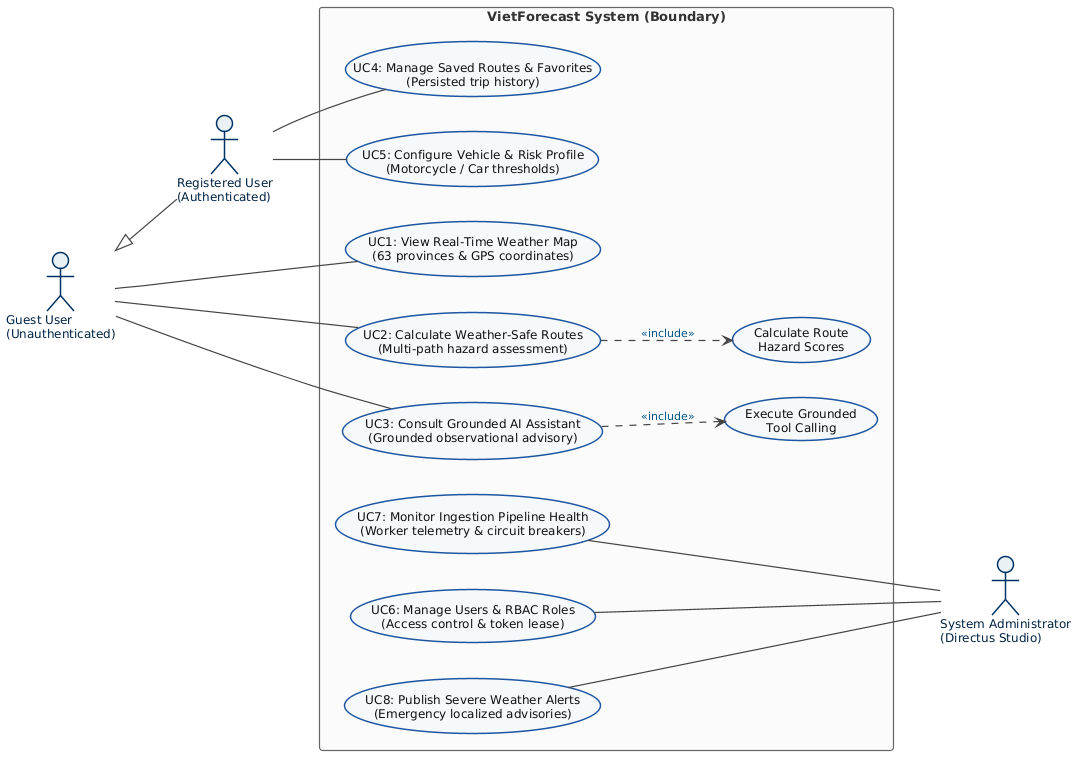
\includegraphics[width=0.95\textwidth]{figures/usecase.png}
\caption{Sơ đồ ca sử dụng tổng quan hệ thống VietForecast theo chuẩn UML 2.5.}
\label{fig:global_use_case_vi}
\end{figure}

\subsection{Bảng tổng hợp đặc tả các ca sử dụng}
Bảng~\ref{tab:use_case_summary_vi} tổng hợp danh mục toàn bộ tám ca sử dụng cốt lõi của hệ thống VietForecast cùng hai ca sử dụng phụ thuộc, phân loại theo nhóm tác nhân và mô tả mục tiêu nghiệp vụ tương ứng:

\begin{table}[H]
\centering
\small
\caption{Bảng tổng hợp đặc tả các ca sử dụng của hệ thống VietForecast.}
\label{tab:use_case_summary_vi}
\begin{tabularx}{\textwidth}{l p{3.4cm} p{2.6cm} X}
\toprule
\textbf{Mã} & \textbf{Tên ca sử dụng} & \textbf{Tác nhân} & \textbf{Mục tiêu và luồng xử lý chính} \\
\midrule
UC1 & Tra cứu bản đồ thời tiết & Guest User, Registered User & Hiển thị các lớp phủ thời tiết thời gian thực tại 63 tỉnh thành hoặc tọa độ định vị GPS. \\
\midrule
UC2 & Tính toán lộ trình an toàn & Guest User, Registered User & Khai phá ba lộ trình thay thế, tính toán ma trận điểm rủi ro và xếp hạng tuyến an toàn thời tiết nhất. Bao gồm ca sử dụng phụ thuộc tính điểm rủi ro. \\
\midrule
UC3 & Trợ lý đàm thoại AI & Guest User, Registered User & Hỗ trợ hỏi đáp tự nhiên bằng tiếng Việt; tự động kích hoạt gọi hàm kiểm chứng dữ liệu trạm quan trắc để ngăn chặn ảo giác thông tin. \\
\midrule
UC4 & Quản lý lộ trình ưa thích & Registered User & Lưu trữ lịch sử di chuyển, danh bạ điểm đến quen thuộc và cấu hình tuyến đường ưu tiên vào cơ sở dữ liệu. \\
\midrule
UC5 & Thiết lập cấu hình rủi ro & Registered User & Tùy biến loại phương tiện (xe máy, ô tô) và cấu hình các trọng số nhạy cảm cá nhân cho các yếu tố khí tượng. \\
\midrule
UC6 & Quản lý người dùng & System Administrator & Quản trị danh sách tài khoản, giám sát phân quyền RBAC và kiểm soát phiên đăng nhập thông qua Directus Studio. \\
\midrule
UC7 & Giám sát đường ống dữ liệu & System Administrator & Theo dõi nhịp tim của worker thu thập dữ liệu, giám sát trạng thái circuit breaker và kiểm tra tỷ lệ làm mới cache. \\
\midrule
UC8 & Phát hành cảnh báo khẩn & System Administrator & Soạn thảo, phê duyệt và phát sóng thông điệp cảnh báo thời tiết cực đoan tới người dùng trong khu vực ảnh hưởng. \\
\bottomrule
\end{tabularx}
\end{table}

\subsection{Đặc tả chi tiết các ca sử dụng cốt lõi}
Để làm rõ yêu cầu nghiệp vụ và hành vi tương tác của từng chức năng, chi tiết đặc tả luồng xử lý của các ca sử dụng được trình bày như sau:

\subsubsection{Ca sử dụng UC1: Tra cứu bản đồ thời tiết thời gian thực}
\begin{itemize}
    \item Tác nhân: Khách vãng lai (Guest User), Người dùng đã xác thực (Registered User).
    \item Tiền điều kiện: Thiết bị có kết nối Internet, dịch vụ API Gateway và giao diện bản đồ MapLibre GL sẵn sàng.
    \item Hậu điều kiện: Bản đồ hiển thị chính xác các lớp dữ liệu khí tượng (nhiệt độ, mưa, gió, tầm nhìn) tại địa điểm lựa chọn.
    \item Luồng sự kiện chính:
    \begin{enumerate}
        \item Người dùng truy cập trang chủ hệ thống hoặc nhấn nút định vị vị trí hiện tại qua GPS.
        \item Trình duyệt gửi yêu cầu truy vấn dữ liệu không gian đến API Gateway.
        \item Hệ thống kiểm tra dữ liệu trong bộ đệm Redis; nếu bộ đệm hợp lệ, trả về tức thì; nếu hết hạn, truy vấn trạm quan trắc gần nhất từ cơ sở dữ liệu PostgreSQL/PostGIS.
        \item Giao diện hiển thị các chỉ số thời tiết chi tiết kèm biểu đồ nhiệt màu trực quan trên nền bản đồ số.
    \end{enumerate}
    \item Luồng ngoại lệ: Nếu người dùng từ chối cấp quyền truy cập GPS, hệ thống mặc định chọn vị trí trung tâm Thủ đô Hà Nội và thông báo cho người dùng.
\end{itemize}

\subsubsection{Ca sử dụng UC2: Tính toán lộ trình an toàn thời tiết}
\begin{itemize}
    \item Tác nhân: Khách vãng lai (Guest User), Người dùng đã xác thực (Registered User).
    \item Quan hệ phụ thuộc: Bao gồm ($\ll$include$\gg$) ca sử dụng tính toán điểm rủi ro thời tiết (Calculate Route Hazard Scores).
    \item Tiền điều kiện: Người dùng nhập điểm xuất phát và điểm đích hợp lệ trong phạm vi lãnh thổ Việt Nam.
    \item Hậu điều kiện: Hệ thống trả về danh sách ba tuyến đường kèm theo điểm rủi ro tổng hợp và cảnh báo thời tiết dọc tuyến.
    \item Luồng sự kiện chính:
    \begin{enumerate}
        \item Người dùng nhập điểm bắt đầu, điểm kết thúc và lựa chọn phương tiện di chuyển (xe máy hoặc ô tô).
        \item Hệ thống gọi dịch vụ OSRM để trích xuất ba phương án lộ trình khả thi (Nhanh nhất, Ngắn nhất, Thay thế).
        \item Hệ thống phân đoạn từng lộ trình thành chuỗi các checkpoint không gian cách đều từ 5 đến 10 km.
        \item Kích hoạt ca sử dụng phụ thuộc tính điểm rủi ro: nội suy thời gian đến dự kiến (ETA) tại từng checkpoint, truy vấn dữ liệu dự báo thời tiết tương ứng và tính toán điểm rủi ro theo sáu chiều nguy cơ.
        \item Hệ thống tổng hợp điểm rủi ro, phân loại tuyến an toàn nhất (Safer Route) và hiển thị trực quan các đoạn nguy hiểm bằng dải màu cảnh báo trên bản đồ.
    \end{enumerate}
    \item Luồng ngoại lệ: Nếu dịch vụ OSRM ngoại vi gặp sự cố hoặc vượt thời gian chờ, hệ thống kích hoạt cơ chế retry; nếu vẫn thất bại, hiển thị thông báo lỗi mạng cho người dùng.
\end{itemize}

\subsubsection{Ca sử dụng UC3: Trợ lý đàm thoại AI có kiểm chứng}
\begin{itemize}
    \item Tác nhân: Khách vãng lai (Guest User), Người dùng đã xác thực (Registered User).
    \item Quan hệ phụ thuộc: Bao gồm ($\ll$include$\gg$) ca sử dụng gọi hàm kiểm chứng dữ liệu trạm quan trắc (Execute Grounded Tool Calling).
    \item Tiền điều kiện: Người dùng gửi câu hỏi liên quan đến thời tiết hoặc hành trình di chuyển vào khung trò chuyện.
    \item Hậu điều kiện: Trợ lý ảo phản hồi câu trả lời tự nhiên bằng tiếng Việt, dựa trên số liệu thực tế được kiểm chứng.
    \item Luồng sự kiện chính:
    \begin{enumerate}
        \item Người dùng nhập câu hỏi bằng ngôn ngữ tự nhiên về tình hình thời tiết hoặc cung đường di chuyển.
        \item API Gateway chuyển tiếp ngữ cảnh đàm thoại đến mô hình Google Gemini 1.5 Flash.
        \item Mô hình phát hiện ý định truy vấn khí tượng và phát sinh lệnh gọi hàm (function calling) với tham số tọa độ và địa danh cụ thể.
        \item Kích hoạt ca sử dụng phụ thuộc gọi hàm: backend thực thi truy vấn dữ liệu quan trắc thực tế của trạm khí tượng tương ứng và gửi kết quả có cấu trúc trở lại cho mô hình.
        \item Mô hình tổng hợp phản hồi đàm thoại súc tích, chính xác dựa trên số liệu đã kiểm chứng, hoàn toàn ngăn chặn hiện tượng ảo giác.
    \end{enumerate}
    \item Luồng ngoại lệ: Nếu địa danh người dùng hỏi không xác định được tọa độ, mô hình đưa ra câu hỏi làm rõ để người dùng cung cấp thêm thông tin vị trí.
\end{itemize}

\subsubsection{Ca sử dụng UC4: Quản lý lộ trình và địa điểm ưa thích}
\begin{itemize}
    \item Tác nhân: Người dùng đã xác thực (Registered User).
    \item Tiền điều kiện: Người dùng đã đăng nhập vào hệ thống với phiên làm việc hợp lệ.
    \item Hậu điều kiện: Thông tin lộ trình hoặc địa chỉ yêu thích được lưu trữ thành công vào hồ sơ cá nhân.
    \item Luồng sự kiện chính:
    \begin{enumerate}
        \item Người dùng nhấn nút lưu lộ trình vừa tìm kiếm hoặc thêm địa điểm quen thuộc vào danh bạ cá nhân.
        \item Ứng dụng gửi yêu cầu lưu trữ dữ liệu kèm theo cookie phiên bảo mật HttpOnly tới API Gateway.
        \item API Gateway xác thực tính hợp lệ của phiên qua Directus và ghi nhận dữ liệu vào bảng cơ sở dữ liệu PostgreSQL.
        \item Danh sách các hành trình đã lưu được cập nhật tức thì trên giao diện quản lý chuyến đi của người dùng.
    \end{enumerate}
    \item Luồng ngoại lệ: Nếu phiên làm việc của người dùng đã hết hạn, hệ thống thông báo yêu cầu đăng nhập lại mà không làm mất dữ liệu lộ trình đang mở.
\end{itemize}

\subsubsection{Ca sử dụng UC5: Thiết lập cấu hình phương tiện và ngưỡng nhạy cảm rủi ro}
\begin{itemize}
    \item Tác nhân: Người dùng đã xác thực (Registered User).
    \item Tiền điều kiện: Người dùng đã đăng nhập vào tài khoản cá nhân.
    \item Hậu điều kiện: Bộ tham số trọng số rủi ro cá nhân hóa được cập nhật và áp dụng cho các lần tìm kiếm lộ trình tiếp theo.
    \item Luồng sự kiện chính:
    \begin{enumerate}
        \item Người dùng truy cập trang cài đặt cấu hình an toàn di chuyển.
        \item Lựa chọn loại phương tiện mặc định (xe máy, ô tô) và tinh chỉnh các thanh trượt ngưỡng nhạy cảm với lượng mưa, vận tốc gió giật hoặc khoảng cách tầm nhìn.
        \item Người dùng nhấn xác nhận lưu cấu hình.
        \item Hệ thống cập nhật các trọng số vào bảng thuộc tính người dùng; các thuật toán tính điểm lộ trình sau đó sẽ tự động áp dụng ma trận trọng số này.
    \end{enumerate}
    \item Luồng ngoại lệ: Nếu người dùng nhập giá trị tham số nằm ngoài khoảng quy định, hệ thống từ chối cập nhật và hiển thị hướng dẫn nhập liệu hợp lệ.
\end{itemize}

\subsubsection{Ca sử dụng UC6: Quản lý người dùng và phân quyền RBAC}
\begin{itemize}
    \item Tác nhân: Quản trị viên hệ thống (System Administrator).
    \item Tiền điều kiện: Quản trị viên đăng nhập thành công vào giao diện Directus Admin Studio với quyền quản trị tối cao.
    \item Hậu điều kiện: Thông tin người dùng, vai trò hoặc quyền truy cập được cập nhật chính xác trong hệ thống.
    \item Luồng sự kiện chính:
    \begin{enumerate}
        \item Quản trị viên điều hướng đến mục quản lý người dùng trên giao diện quản trị Directus.
        \item Thực hiện các thao tác: duyệt danh sách tài khoản, kích hoạt, tạm khóa người dùng, hoặc gán vai trò quyền hạn (Role-Based Access Control).
        \item Hệ thống ghi nhận toàn bộ lịch sử thao tác vào nhật ký kiểm toán (audit log) để đảm bảo tính minh bạch và an toàn thông tin.
    \end{enumerate}
    \item Luồng ngoại lệ: Hệ thống ngăn chặn hành vi tự xóa tài khoản hoặc tự hạ quyền quản trị của chính tài khoản đang đăng nhập để tránh mất quyền điều hành.
\end{itemize}

\subsubsection{Ca sử dụng UC7: Giám sát đường ống thu thập dữ liệu}
\begin{itemize}
    \item Tác nhân: Quản trị viên hệ thống (System Administrator).
    \item Tiền điều kiện: Quản trị viên truy cập trang tổng quan giám sát hệ thống.
    \item Hậu điều kiện: Trạng thái vận hành của các dịch vụ ngầm và đường ống dữ liệu được cập nhật đầy đủ.
    \item Luồng sự kiện chính:
    \begin{enumerate}
        \item Quản trị viên kiểm tra bảng điều khiển hiển thị trạng thái của tiến trình Integration Worker.
        \item Hệ thống cung cấp thông tin nhịp tim (heartbeat), thời điểm cập nhật dữ liệu gần nhất, trạng thái circuit breaker và tỷ lệ thành công của các yêu cầu gửi đến nhà cung cấp thời tiết ngoại vi.
        \item Nếu phát hiện dấu hiệu bất thường (như dữ liệu quan trắc trễ quá 60 phút hoặc lỗi API liên tiếp), hệ thống hiển thị cảnh báo mức đỏ.
    \end{enumerate}
    \item Luồng ngoại lệ: Khi đường ống chính gặp sự cố, hệ thống cho phép quản trị viên kích hoạt chế độ tải dữ liệu thủ công từ nguồn dự phòng.
\end{itemize}

\subsubsection{Ca sử dụng UC8: Phát hành bản tin cảnh báo thời tiết khẩn cấp}
\begin{itemize}
    \item Tác nhân: Quản trị viên hệ thống (System Administrator).
    \item Tiền điều kiện: Quản trị viên ghi nhận thông tin thiên tai, bão lũ hoặc hiện tượng thời tiết nguy hiểm cần thông báo khẩn cấp.
    \item Hậu điều kiện: Bản tin cảnh báo được lưu vào cơ sở dữ liệu và hiển thị nổi bật trên bản đồ số của tất cả người dùng trong vùng ảnh hưởng.
    \item Luồng sự kiện chính:
    \begin{enumerate}
        \item Quản trị viên mở biểu mẫu tạo thông báo khẩn cấp trên giao diện quản trị.
        \item Nhập nội dung cảnh báo, chọn mức độ rủi ro (vàng, cam, đỏ) và xác định phạm vi địa lý bị ảnh hưởng (danh sách tỉnh thành hoặc đa giác tọa độ).
        \item Quản trị viên nhấn nút phê duyệt phát hành bản tin.
        \item Hệ thống lưu trữ bản tin và đồng bộ trạng thái để kích hoạt biểu tượng cảnh báo tức thời trên giao diện ứng dụng của người dùng.
    \end{enumerate}
    \item Luồng ngoại lệ: Nếu quản trị viên chưa chọn phạm vi địa lý hoặc nội dung cảnh báo còn để trống, hệ thống yêu cầu hoàn thiện đầy đủ các trường thông tin bắt buộc trước khi phát sóng.
\end{itemize}

\section{Kiến trúc hệ thống mức khái niệm}
Để hiện thực hóa các yêu cầu chức năng và phi chức năng đã đề ra, đồng thời bảo đảm tính toàn vẹn và độ tin cậy của dịch vụ, hệ thống VietForecast được mô hình hóa theo sơ đồ ngữ cảnh C4 (C4 Model Level 1 -- System Context) như thể hiện trong Hình~\ref{fig:conceptual_overview_vi}. Mô hình phân định rõ ranh giới hệ thống, các nhóm tác nhân tương tác và các dịch vụ đám mây ngoại vi:
\begin{itemize}
    \item Nhóm tác nhân người dùng (Platform Users): Bao gồm người tham gia giao thông (Commuter / Traveler) truy cập hệ thống qua ứng dụng web để tra cứu thời tiết, tìm kiếm lộ trình an toàn và tương tác với trợ lý AI; cùng quản trị viên hệ thống (System Administrator) thực hiện cấu hình vận hành, giám sát đường ống dữ liệu và phát hành các bản tin cảnh báo khẩn cấp qua giao diện Directus Admin Studio.
    \item Nền tảng trung tâm VietForecast (Core Software System): Là thành phần cốt lõi của giải pháp, chịu trách nhiệm tiếp nhận và xử lý các yêu cầu từ phía người dùng thông qua API Gateway hiệu năng cao. Hệ thống tự động điều phối tiến trình thu thập và chuẩn hóa dữ liệu từ các trạm khí tượng, vận hành động cơ đánh giá rủi ro đa chiều, thực thi thuật toán tìm kiếm lộ trình an toàn thời tiết và cung cấp giao diện hội thoại thông minh có kiểm chứng dữ liệu thực tế.
    \item Các dịch vụ đám mây ngoại vi (External Cloud Services): Bao gồm dịch vụ WeatherAPI cung cấp dữ liệu quan trắc thời gian thực và dự báo số trị chuẩn WMO; dịch vụ OSRM kết hợp bản đồ OpenStreetMap \cite{haklay2008openstreetmap} cung cấp đồ thị mạng lưới đường bộ và thuật toán tìm đường cơ sở; cùng mô hình ngôn ngữ lớn Google Gemini 1.5 Flash đóng vai trò khối suy luận ngôn ngữ tự nhiên được kiểm soát chặt chẽ thông qua giao thức gọi hàm nội bộ.
\end{itemize}

\begin{figure}[H]
\centering
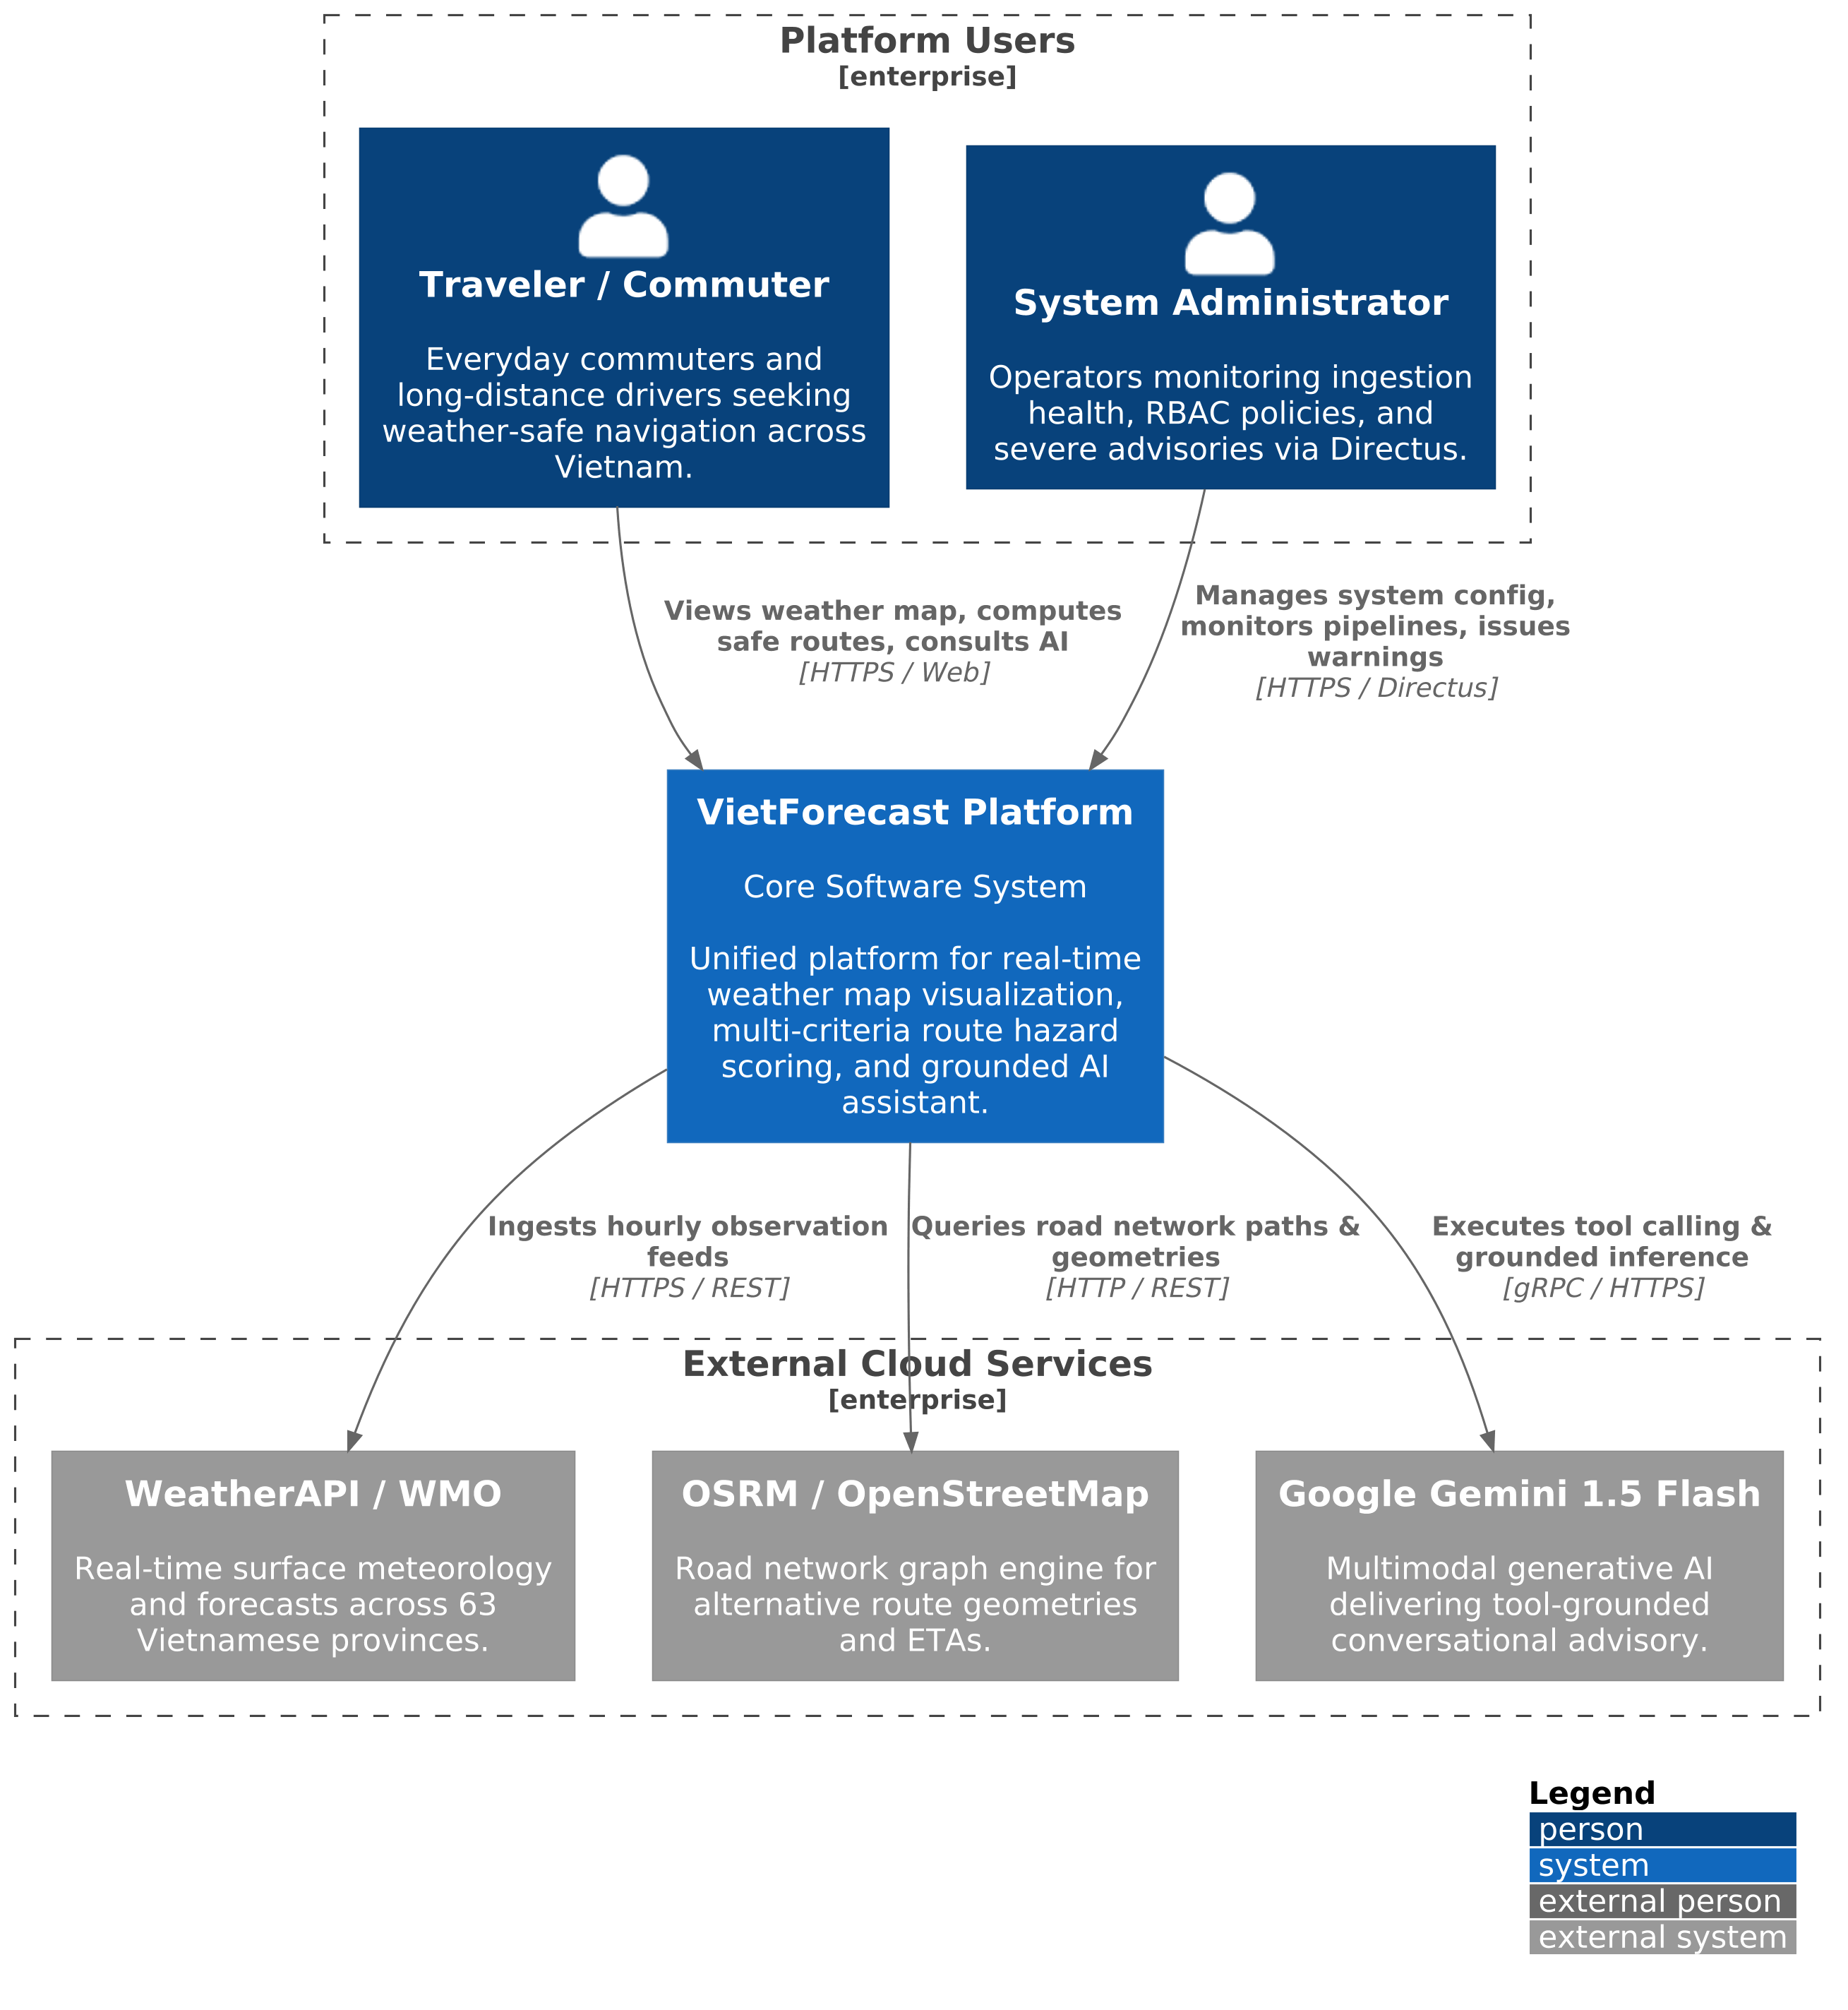
\includegraphics[width=0.92\textwidth]{figures/c4_context.png}
\caption{Sơ đồ ngữ cảnh hệ thống VietForecast theo mô hình C4 (C4 Context Diagram).}
\label{fig:conceptual_overview_vi}
\end{figure}


